 \chapter{Important Concepts and Variable Definitions}\label{Important_concepts_chapter}
 
 \section{Jets}
 A jet can be defined as a high energy shower of stable particles that comes from fragmentation of quarks or gluons. The initial quarks and gluons in the process are known as ``initial partons''.
 Due to that initial partons are colour charged, they can not be isolated singularly (this phenomenon is called ``colour confinement''). Since it is not possible for coloured particles to be isolated 
 they must go through a non-perturvative process that converts them into colour neutral particles. This process is called ``hadronization'' and there are different models to explain it. According to 
 the string model, the confining nature of strong interaction increases the potential colour in a proportional way as the distance between the initial partons. When the distance reaches a certain 
 critical value it is energetically favourable to produce a quark pair from the vacuum. Finally, by this proccess the inital colour charged particles are converted into bound colour-singlet hadronic 
 states. \\
 %Citar libro: Particle detectors Calus GRupen and Boris shwartz
 
 Despite jets may display a structure with properties that could indicate which were the initial partons interacting, they are hard to study individually when there is a numerous quantity of them
 in an event. The former is because it is almost imposible to associate all particles in an event final state to a single initial parton. The reconstruction of jets depends of elements like the 
 fragmentation process, detectors effects, among others. Thus, there exist algorithms which cluster some particles in a final state so that it is possible to determine properties as 4-momentum 
 and jet shapes. The objective of these algorithms is to determine the inital interacting partons and approximate its directions and energies. \\
 
 According to the reconstruction algorithms we can define a jet at three different levels. At parton level a jet can be understood as a quark or a gluon. At hadronic level can be referred to the
 hadrons produced due to the hadronization process, like kaons or pions. Finally, at a detector level a jet can be understood as a set of reconstructed tracks spatially associated with energy 
 deposited in the calorimeters. The reconstuction algorithms that are going to be used for this analysis consist in the use of mathematical cones that enclose the regions where a large quantity
 of particles are 
 detected. The radius of the cone must be large enough to enclose all the particles comming from the initial quark or gluon, and must be small enough to not include other particles that belong to a 
 different jet. The three level definitions just mentioned are illustrated in Figure \ref{Jets_definitions}. In this figure the mathematical cones used for the reconstruction of a jet is also showed.
 %Citar tesis Luis Alfredo
 
 %Citar figura https://phys.org/news/2012-07-jets-cms-energy-scale.html
 
 \begin{figure}[h] 
 \centering
 \caption{Description of a jet at three different levels: partonic, hadronic and detector.}
 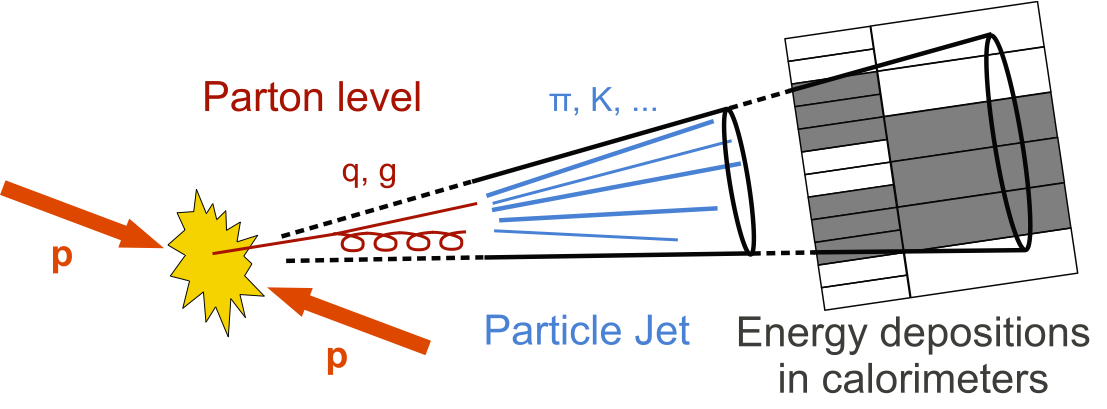
\includegraphics[width=0.75\textwidth]{./Capitulos/VariableDefinitions/jets_definitions}  
 \label{Jets_definitions}
 \end{figure}
 
 \section{Cross Section and Luminosity}
 
 In High Energy Physics, the cross section $\sigma$ represents the probability that a given physical proccess occurs. This quantity is proportional to the energy of the event production. The unit 
 used for cross sections is the bar (1b = $10^{-28} \text{m}^2$). The number of expected events of a certain interaction in a fixed target experiment is proportional to its cross section, the particles flux, and the
 number of atoms per cubic meter in the target multiplied by the lenght. The inverse of the number of atoms per area is called ``target constant $F$'' and it has the dimesion of an area. Thus, it 
 is possible to make an estimation of the number of interactions per second using:
 
 %citar libro data analysis techniques for high energy physics
 \begin{equation}
 \label{luminosity}
  \frac{N_{events}}{s} = \sigma \times \frac{N_{flux}/s}{F} = \sigma \times Luminosity
 \end{equation}

 In the Equation \ref{luminosity} we defined the concept of luminosity, which is a measure of sensitivity and depends on the energy and on the beam dynamics.  The luminosity is a quantity that is used to 
 describe the performance of a particle accelerator. It has units of the inverse of cross section, which is know as inverse barns $fb^{-1}$ and it is equivalent to $(1 fb = 10^{-28} m^2)$. 
 In particle colliders the 
 luminosity depends on different variables such as the number of particles per bunch $N_b$, the number of bunches in each beam $\kappa_b$, the revolution frequency $f$ at the storage ring and the beam radii 
 $R$ of the bunches at the crossing point:
 
 \begin{equation}
  L = \frac{N_b^2 f \kappa_b}{4\pi R^2} 
 \end{equation}

 \section{Pseudorapidity}
 %GENERALIZAAAAAAAAAAAAAAAAAAAAAAAAAAAAAAAAAAAAAAAAAAAAAAAAAAAAAAAAR
 
 The variable pseudorapidity is defined as a parametrization of the CMS detector coordinates. These coordinates are ilustrated in the Figure \ref{CMSCoordinates}:
 
 \begin{figure}[h]
 \centering
 \caption{CMS detector coordinates}
 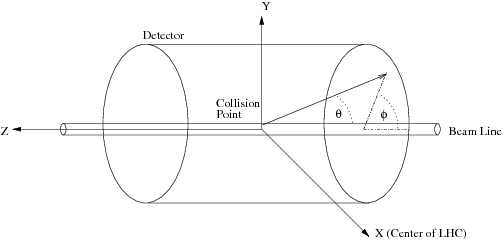
\includegraphics[width=0.75\textwidth]{./Capitulos/VariableDefinitions/CMS_coordinates}  
 \label{CMSCoordinates}
 \end{figure}

%CITAR GRAFICAAAA

The origin of the CMS coordinates coincides with the point in which a collision occurs in the detector. 
The polar angle is described by the parameter $\theta$ and it is measured with respect to the z axis.
The azimuthal angle is denoted by $\Phi$ and it is measured in the xy plane from the x axis. The pseudorapidity is defined in terms of the polar angle as:

\begin{equation}
 \eta \equiv - \ln \left( \tan (\theta /2 ) \right)
\end{equation}

 The motivation to define and use this variable is that while $\Delta \theta$ is not a Lorentz invariant $\Delta \eta$ is. Moreover, the quantity of particles depending on the variable $\eta$
 is approximately uniform in a cilindrical detector. 
 
  
 \section{$p_T$ and $\vec{E_T^{miss}}$}

 The quantity $p_T$ is the transversal momentum and it is the projection of the linear momentum onto the xy plane. This variable is used instead of the linear momentum because the initial beams
 are moving just in the z axis (the initial momentum in the xy plane is zero), so when a collision is produced the interesting effects occur in the transverse plane.\\
 %the particles adquiere momentum in the xy plane. 
 
 As it was already mentioned, the momentum in the tranverse plane is zero before the collision. Since the tranverse momentum has to be conserved, after the collision it must also be zero. We can write
 the total momentum as the sum of the particles that are detected (visible particles) and the ones that are not detected (invisible particles), which can be expressed as:
 
 \begin{equation}
  0 = \sum_{i=1}^N \vec{P_T(i)} = \sum_{j=1}^M \vec{P_T(j)}^{visible} + \sum_{k=M}^{N-M} \vec{P_T(k)}^{invisible}
 \end{equation}

%CITAAAAAAAAAAAAAAAR

 The last equation motivates the definition of a variable called ``Missing transverse energy'' ($\vec{E_T^{miss}}$), which is defined as the sum of the transverse momentum of the invisible
 particles:
 
 \begin{equation}
  \vec{E_T^{miss}} \equiv \sum_{k=M}^{N-M}\vec{P_T(k)}^{invisible} = - \sum_{j=1}^M  \vec{P_T(j)}^{visible}
 \end{equation}

 
 \section{Displaced Vertices and Impact Parameter}
The vertex of a track is a variable of importance because it can be used to determine the position of the point of interaction and the momentum vector of the tracks emerging from the vertex. The 
vertex fit can also be used to check the association of tracks to a vertex, in other words, to determine if a track actually originates from a certain vertex. In order to determine the direction
of the track connecting a primary and a secondary vertex we have to find the position of the secondary vertex. Some particles can pass through the detector without leaving tracks. However,
when these undetected particles decay, the particles produced can be observed because they leave tracks on the detector. The point in which the product particles are detected is called a secondary 
vertex, and it is said that it is a displaced vertex. Figure \ref{Displaced_vertex} shows a sketch of a displaced vertex, where the path of the undetected particle is represented by a dotted line.

 % Imagen tomada Displaced Vertex: https://indico.cern.ch/event/149404/contributions/1388848/attachments/149638/211969/azuma_berkeley_111020_v05.pdf
 % Imagen Impact parameter: http://www.quantumdiaries.org/2011/06/10/to-b-or-not-to-bbar-b-tagging-via-track-counting/
  
 \begin{figure}[h] 
 \centering
 \caption{Scheme of a displaced vertex}
 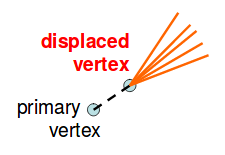
\includegraphics[width=0.4\textwidth]{./Capitulos/VariableDefinitions/Displaced_vertex} 
 \label{Displaced_vertex}
 \end{figure}
 
The impact parameter is defined as the closest distance between the vertex and the points of the track. A visualization of this is showed in Figure \ref{Impact_parameter}. In this image the track is represented by the blue dotted line, and the impact parameter by the red line. It can be seen that the impact parameter line forms a right angle with the track. Using this characteristic it is possible to identify in a unique way the closest point of approach of the track to the vertex.


 \begin{figure}[h] 
 \centering
 \caption{Scheme of the impact parameter variable}
 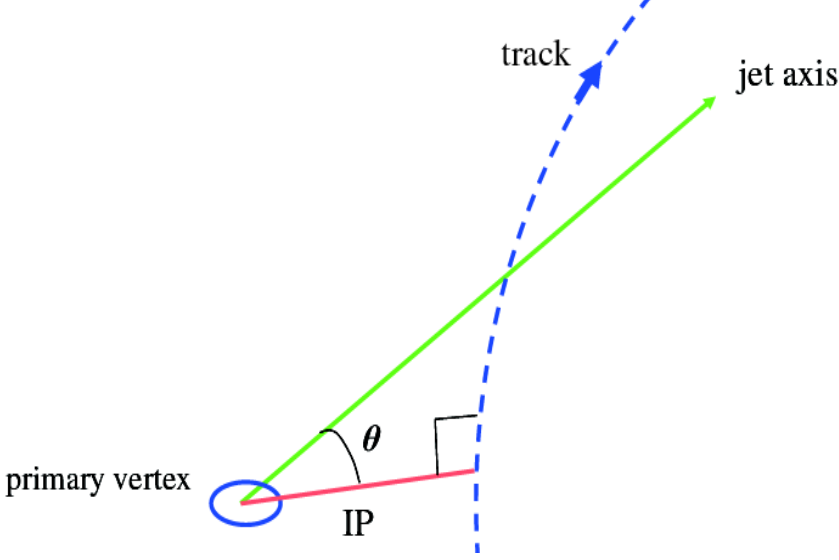
\includegraphics[width=0.7\textwidth]{./Capitulos/VariableDefinitions/impactParameter}  
 \label{Impact_parameter}
 \end{figure} 

 
 
 
 
 
 
 
 
 
 
 
 
 
 
 
 
 
 
 